\section{Mesh Fitting}
\label{sec:fitting}

We pose mesh fitting to 3D point data as finding the most likely surface that would have generated those points.  By incorporating prior surface assumptions, the fitting process estimates a continuous surface from discrete points that can eliminate much of the measurement noise.  Methods that fit mesh models to 3D points often minimize the perpendicular distance of points to facets [REF].  This makes sense when point-cloud noise is equal in all directions or else the point noise is small compared to the facets.  For our data the measurement noise is large and is not equal in all directions, but rather is along the depth camera rays.  Hence the focus of this section is to develop a mesh fitting method that minimizes these pixel depth errors along the pixel rays.

In this paper we define a mesh in a $2$D image space and project it into $3$D.  This is more limiting than full $3$D meshes as it models only the surface portions visible from the sensor, but it also provides a number of advantages.  Compared to methods that fit prior surface models to depth maps [ref], need to search of the space of poses, scales and distortions of the model with the chance of finding local minima.  Compared to voxel-based models with implicit surfaces [ref], our method can better incorporate pixels uncertainties and surface priors, as well as having fewer discretization artifacts.  In addition our method can naturally incorporate detailed features from the high-resolution color camera, and reflectivity information from the IR reflectance image.

\subsection{Notation}

A vertex, $\vertex$, is a vector in $3$D.  In a given camera coordinate system, it projects onto a pixel on the unit focal-length image-plane $\hvertex=(u,v,1)^\top$, where the `` $\tilde{\text{ }}$ '' indicates a homogeneous vector, and $u$ and $v$ are the coordinates in this plane.  Now $\hvertex$ defines a ray from the camera origin, and the original vertex is obtained by scaling the image-plane vertex by its depth, $\lambda$, along the ray, namely: $\vertex = \lambda\hvertex$. 

\subsection{Facet Model}

Mesh fitting for an individual facet is illustrated in Figure~\ref{fig:facet}.  The $2$D vertices and edge connections are determined in an image, in this case the color image although it could be the depth image, as described in section~\ref{sec:mesh}.  If these vertices lie on a feature of the target leaf, such as its edge, we know that that those $3$D features like somewhere along the rays emanating from camera origin through those vertices.  Hence a triangular facet approximation to the object surface will have vertices on these three rays.  

\begin{figure}
\begin{center}
   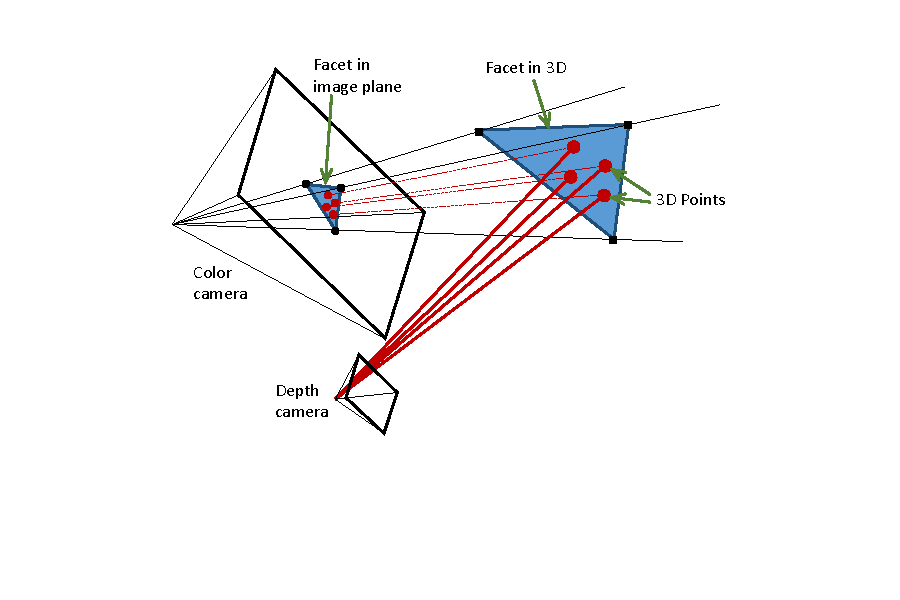
\includegraphics[trim=80 70 70 20,clip,width=0.95\linewidth]{Figures/pointFittingConcept}
\end{center}
   \caption{The parallel and adjacent color and depth cameras are shown as pyramids denoting their fields of view, and their size difference illustrates their relative resolutions.  Three vertices in a color image define the rays on which the vertices of the corresponding $3$D object facet must lie.  This facet is fit using the the $3$D points projected out from the depth camera.}
\label{fig:facet}
\end{figure}

The next step is to associate depth measurements with the facet.  Pixels in the depth camera are projected along their rays out into $3$D.  The resulting $3$D points that lie within the facet pyramid (defined by these rays through its vertices) will project into the $2$D facet in the color image.  Hence it is straightforward to associate $3$D points with mesh facets.  

To estimate the facet parameters from depth measurements we will express the depth points as a linear function of the vertices of its facet.  We make a local orthographic approximation for the projection of a facet.  This will be a good approximation as long as the facet size is small compared to is depth from the camera, which is true for most applications.  Given this assumption, the coordinates of a point $\point$ lying on a facet can be expressed as a linear combination of the three vertex coordinates $\vertex_a$, $\vertex_b$ and $\vertex_c$ as follows:
\beq  %see PlantMacros.tex
\point = \alpha_a \vertex_a + \alpha_b \vertex_b + \alpha_c \vertex_c. \label{eq:point}
\eeq
The coefficients $\alpha_a$, $\alpha_b$ and $\alpha_c$ are defined in Figure~\ref{fig:triangle}.  Substituting in depth-scaled homogeneous vectors, and taking the third row, we obtain an equation for the point depth, $\lambda_{p}$:
\beq
\lambda_{p} = \alpha_a \lambda_a + \alpha_b \lambda_b + \alpha_c \lambda_c, \label{eq:pointdepth}
\eeq
where $\lambda_a$ is the depth of $\vertex_a$ and so forth.  

\begin{figure}
\begin{center}
   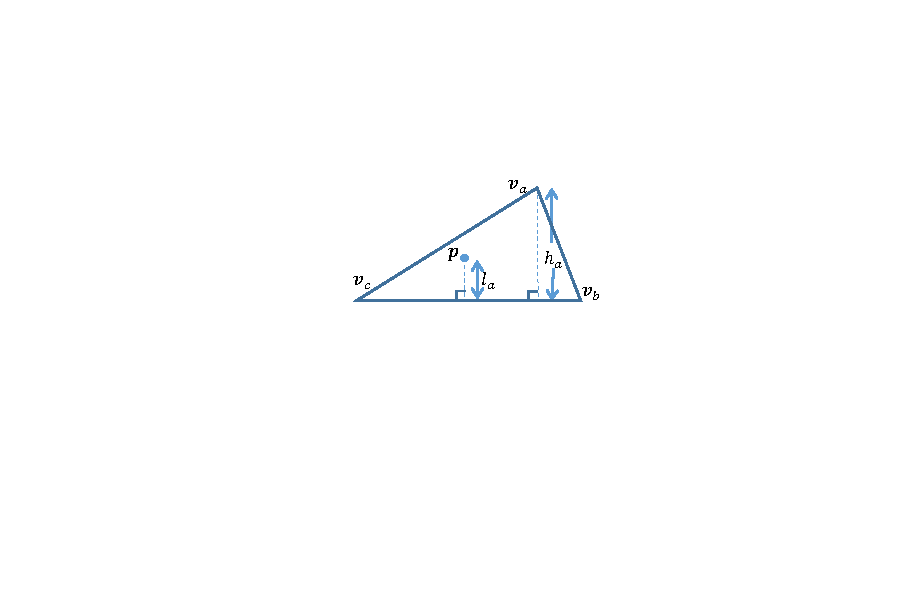
\includegraphics[trim=150 140 140 80,clip,width=0.75\linewidth]{Figures/TriangleParameterization}
\end{center}
   \caption{The coordinates of a point on a facet described by Eq.~(\ref{eq:point}) are the weighted linear sum of the three vertex coordinates.  The weight, $\alpha_a$, for vertex $\vertex_a$ is given by $\alpha_a = \frac{l_a}{h_a}$, the ratio of its perpendicular distance $l_a$ to the opposite edge to the vertex perpendicular distance $h_a$.  Analogous expressions describe $\alpha_b$ and $\alpha_c$. }
\label{fig:triangle}
\end{figure}

\subsection{Least Squares Depth}

Equation (\ref{eq:pointdepth}) gives the depth of one point in terms of its facet vertices.  For mesh with many facets and a measurement with many depth points, a vector of pixel depths, $\vlambda_d$, and vector of vertex depths, $\vlambda_v$, are related with a coefficient matrix, $A$, containing the appropriate $\alpha$'s:
\beq
\vlambda_d = A \vlambda_v. \label{eq:linearmesh}
\eeq
Given a measurement vector of point depths, $\bar{\vlambda}_d$, expressed in the color camera coordinates, the error vector between these depths and the corresponding mesh points is: $\bar{\vlambda}_d - A \vlambda_v$.  Notice that this error is along the color camera rays which to a good approximation are parallel to the depth camera rays, and thus the noise model in Eq.~(\ref{eq:sigma}) applies.  This justifies the following weighted squared error formulation:
\beq
E_{depth} = \| W \bar{\vlambda}_d - W A \vlambda_v \|^2, \label{eq:meshleastsquares}
\eeq
where $W$ is a diagonal matrix containing the inverse standard deviation, $\sigma^{-1}$, from Eq.~(\ref{eq:sigma}).

\subsection{Shape from Shading}

The depth camera measures IR reflectance in addition to depth at each pixel.  Since the reflectance depends on the angle between the surface normal and the incident ray from the IR illuminator, the reflectance image can provide useful cues on the object surface.  Shape from shading techniques model this dependence on the surface normal, along with additional surface assumptions such as smoothness, to estimate the normals and integrate an object surface [REF].  However the real world practicality of these methods has been limited since they generally require a single known light source position illuminating a Lambertian surface, the integration is sensitive to noise, and shape is obtained only up to a scale factor.  Fortunately our application satisfies the key requirements of Shape from Shading, (we have a known light source and leafs are modeled well as Lambertian surfaces~\cite{Chelle2006219}), and our mesh model provides additional information that removes the need to integrate noisy surface normals.  This section describes our use of Shape from Shading to improve shape recovery.

\begin{figure}
\begin{center}
   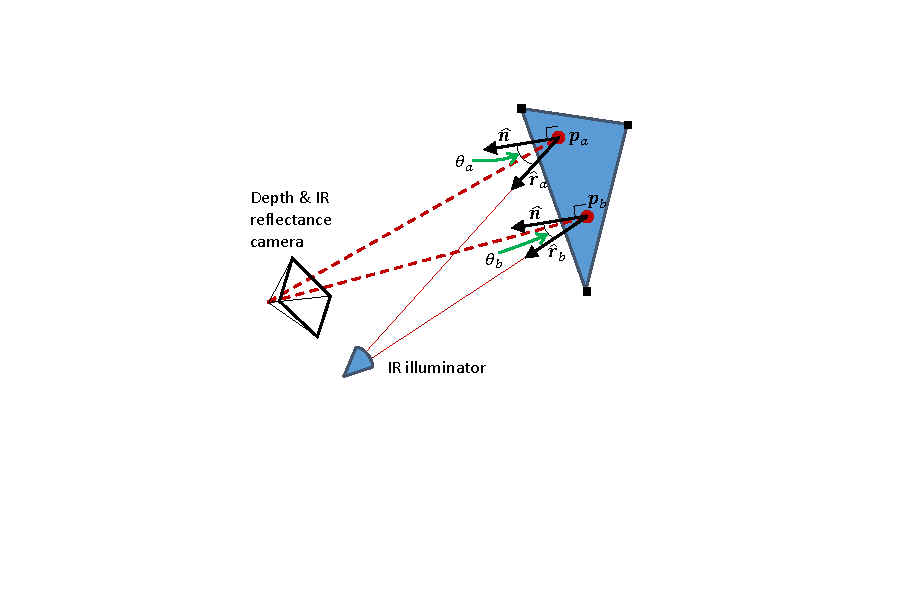
\includegraphics[trim=100 100 100 40,clip,width=0.95\linewidth]{Figures/ShapeFromShading}
\end{center}
   \caption{Our geometric model for the reflectance image.  At each depth point the intensity of the reflectance image will depend on a number of factors including the angle between the facet normal and the ray to the illuminator shown for two points as $\theta_a$ and $\theta_b$. }
\label{fig:shapefromshading}
\end{figure}

\subsubsection{Reflectance Modeling}

We build a simplified bidirectional reflectance model to explain the pixel values, $R_i$, of the IR reflectance image, shown in Figure~\ref{fig:plantnoise}($b$).  This model for pixel $i$ is:
\beq
R_i = \frac{I_i}{r_i^h}\ray_i\cdot\normal_i \rho s_i.\label{eq:reflectanceinit}
\eeq
Here $I_i$ is the intensity of the ray from the IR illuminator.  For a source emanating in all directions this would decrease with a factor of $\frac{1}{r_i^2}$, but a focused beam the decrease may be less, and we model the decay power with $h$.  Under a Lambertian assumption the reflected beam is given by $\ray_i\dot\normal_i \rho = \cos(\theta_i) \rho$ where $\theta_i$ is the angle between the ray to source $\ray_i$ and the surface normal $\normal_i$, and $\rho$ is the albedo.  Finally the sensor scales the incoming beam with a factor $s_i$.  This model can be simplified further by merging some of the unknown parameters.  We define a pixel gain $g_i = \log(I_i \rho s_i)$, and the resulting model is:
\beq
R_i = \frac{ \exp(g_i) \cos(\theta_i)}{r_i^h}. \label{eq:reflectance}
\eeq

The unknown parameters in Eq.~\ref{eq:reflectance} are $g_i$ and $h$, and they can be calibrated as follows.   Depth and reflectance images are taken of a flat, uniform albedo target at various depths and inclinations.  




\subsection{Regularization}

Prior models on surface properties can be incorporated into the mesh via regularization and in so doing reduce the impact of noise.  Membrane energy is a well-used function in mesh optimization~\cite{Kobbelt:1998} and can be minimized using the discrete Laplacian operator.  Here we use Laplacian smoothing due to its simplicity and good performance~\cite{Kobbelt:1998,Ohtake2001789,Chen2005376}, although we modify it to accommodate image-based edge information.  In addition, rather than apply Laplacian smoothing after the fact, entailing an iterative optimization~\cite{Kobbelt:1998}, we show that Laplacian smoothing can be incorporated directly into the least squares mesh estimation.  This has a number of  advantages over application after the initial mesh estimation.  First the smoothing penalty is traded off against measurement error rather than vertex offset.  Second, the due to our ray constraints on the vertices we are able to derive a linear solution with not need to iterate.  Finally  when the regularization components are added to Eq.~(\ref{eq:meshleastsquares}) they ensure that the solution is well-posed even when some of the facets have no depth points in them.

Laplacian smoothing uses an umbrella-operator~\cite{Kobbelt:1998} on a vertex, $\vertex$, and its neighbors $\vertex_i\in\mathcal{N}(\vertex)$,
\beq
\vect{u}(\vertex) = \frac{1}{n}\sum_{\vertex_i\in\mathcal{N}} \vertex_i - \vertex,\label{eq:umbrella}
\eeq
for $n$ neighbors as illustrated in Figure~\ref{fig:laplacian}.  In our model the vertices lie along known rays and so this operator can be expressed as a function of the vertex depth: $\vect{u}(\lambda) = \frac{1}{n}\sum_{i\in\mathcal{N}} \lambda_i \hvertex_i - \lambda\hvertex$.  The squared magnitude $\|\vect{u}(\lambda)\|^2$ is a natural penalty term as it captures a discrete form of the membrane energy.  Summing this over all vertices and arranging the known $\hvertex$ components into a single matrix $U$, we obtain
\beq
E_{reg} = \| U \vlambda \|^2.
\eeq

\begin{figure}
\begin{center}
   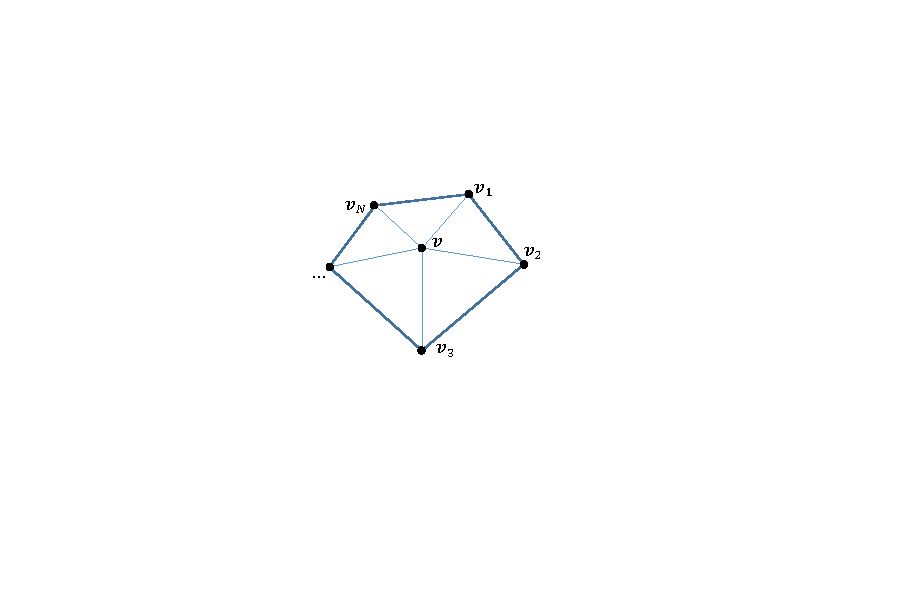
\includegraphics[trim=100 110 140 90,clip,width=0.8\linewidth]{Figures/LaplacianFacets}
\end{center}
   \caption{In discrete form the Laplacing is implemented as an umbrella operator, Eq.~(\ref{eq:umbrella}), over a vertex $\vertex$ and its first neighbors.}
\label{fig:laplacian}
\end{figure}


